\documentclass[a4paper, 12pt]{article}
\usepackage{graphicx} % Required for inserting images
\usepackage{amsthm}
\usepackage{dsfont}
\usepackage{amsmath}
\usepackage{tikz}
\usetikzlibrary{arrows}
\theoremstyle{definition}
\newtheorem{thm}{Theorem}[section]
\newtheorem{defn}[thm]{Definizione}
\newtheorem{lem}{Lemma}[thm]
\newtheorem{cor}{Corollary}[thm]
\newtheorem{prop}{Proposition}[thm]
\newtheorem{rem}{Remark}[thm]
\newtheorem{ill}{Illustration}[thm]

\usepackage[
a4paper,
top=2cm,
bottom=2cm,
left=2cm,
right=2cm,
heightrounded,
bindingoffset=5mm
]{geometry}

\title{Appunti di Geometria e algebra lineare}
\author{Sofia Riva}

\begin{document}

\maketitle

\newpage
\section{Matrici}
\noindent Prima di definire una matrice è necessario conoscere la definizione di prodotto cartesiano:
\begin{defn}
Dati due insiemi \( A \) e \( B \), il prodotto cartesiano \( A \times B \) è l'insieme delle coppie ordinate \( (a,b) \) con \( a \in A \) e \( b \in B \).
\end{defn}
\noindent Vogliamo ora descrivere una funzione che abbia come dominio un prodotto cartesiano di insiemi finiti, e come codominio un insieme numerico o campo $\mathds{K}$
\begin{defn}
Una matrice \( A \) è una funzione \( A: [m] \times [n] \to \mathds{K} \), dove \( [m] = \{1, 2, \dots, m\} \), \( [n] = \{1, 2, \dots, n\} \) e \( \mathds{K} \) è un campo. Ovvero A è una tabella con $m$ righe e $n$ colonne, contenenti valori in $\mathds{K}$
\end{defn}
\[ 
\boldsymbol{A} = \begin{bmatrix}
a_{11} & a_{12} & ... & a_{1n} \\
a_{21} & a_{22} & ... & a_{2n} \\
... & ... & ... & ... \\
a_{m1} & a_{m2} & ... & a_{mn} \\
\end{bmatrix}
\]

\noindent Scriviamo $M_\mathds{K}(m, n)$ per indicare l'insieme di tutte le matrici con $m$ righe e $n$ colonne, e contenti valori in $\mathds{K}$.
Osserviamo ora alcuni casi particolari
\begin{itemize}
    \item Se \( m = n = 1 \), allora \( M_\mathds{K}(1, 1) = \mathds{K} \).
    \item Se \( m = 1 \) e \( n > 1 \), allora
    \[
    \mathbf{A} = \begin{bmatrix}
    a_{11} & a_{12} & \dots & a_{1n}
    \end{bmatrix}
    \]
    prende il nome di \textit{vettore riga} di lunghezza $n$.
    \item Se \( m > 1 \) e \( n = 1 \), allora
    \[
    \mathbf{A} = \begin{bmatrix}
    a_{11} \\ a_{21} \\ \dots \\ a_{m1}
    \end{bmatrix}
    \]
    prende il nome di \textit{vettore colonna} di altezza $m$.
    \item Se \( m = n \), otteniamo una matrice $\mathbf{A}$ del tipo $M_\mathds{K}(n, n)$. Le matrici di questo tipo si dicono \textit{matrici quadrate} di ordine $n$
\end{itemize}
\noindent Definiamo ora l'uguaglianza tra due matrici:
\[
\mathbf{A} \in M_\mathds{K}(m, n) \hspace{1cm} \mathbf{B} \in M_\mathds{K}(p, q)
\]
\begin{itemize}
    \item[-] se $m \neq p$ oppure $n \neq q$, allora $\mathbf{A} \neq \mathbf{B}$
    \item[-] se $m = p$ e $n = q$, allora $\mathbf{A} = \mathbf{B}$ se e solo se $A(i,j) = B(i,j) $ \hspace{1cm} $ \forall(i,j) \in [m]\times[n]$
    ovvero $a_{ij} = b_{ij} \hspace{0.5cm} \forall{i = 1,\dots,m} \hspace{0.5cm}, \forall{j = 1,\dots,n}$
\end{itemize}
\noindent Possiamo adesso definire la somma tra matrici:
\begin{defn}
    Siano $\mathbf{A}, \mathbf{B} \in  M_\mathds{K}(m, n)$, la sommma  $\mathbf{A} + \mathbf{B}$ restituisce una nuova matrice, che si ottiene sommando gli elementi delle due matrici che occupano le stesse posizioni
\end{defn}
\noindent La somma si fa "posizione per posizione"
\newpage
\noindent Proprietà della somma tra matrici:
\begin{itemize}
    \item \textit{associativa} \hspace{1.5cm} $\forall{\boldsymbol{A,B,C}} \in  M_\mathds{K}(m, n) \hspace{1cm }(\boldsymbol{A + B}) + \boldsymbol{C} = \boldsymbol{A} + (\boldsymbol{B} + \boldsymbol{C})$
    \item \textit{commutativa} \hspace{1.5cm} $\forall{\boldsymbol{A, B}} \in  M_\mathds{K}(m, n) \hspace{1cm} \boldsymbol{A + B = B + A} $
    \item \textit{esistenza dell'elemento neutro} $\exists \underline{O} \in  M_\mathds{K}(m, n)\hspace{0.5cm}t.c\hspace{0.5cm} \boldsymbol{A} + \boldsymbol{\underline{O}} = \boldsymbol{\underline{O}} + \boldsymbol{A} = \boldsymbol{A} $
    \[
    \underline{O} = \begin{bmatrix}
        0 & \dots & 0 \\
        \dots & \dots & \dots \\
        0 & \dots & \dots
    \end{bmatrix}
    \]
    \item \textit{esistenza dell'elemento opposto} $\forall{\boldsymbol{A}} \in M_\mathds{K}(m, n) \hspace{0.5cm} \exists{\boldsymbol{A'}} \in M_\mathds{K}(m, n) \hspace{0.5cm} t.c \hspace{0.5cm} \boldsymbol{A} + \boldsymbol{A'} = \boldsymbol{\underline{0}} $
    \[ l'elemento\hspace{0.2cm} opposto \hspace{0.2cm} di \hspace{0.2cm} \boldsymbol{A} = [a_{ij}] \hspace{0.2cm} \acute{e} \hspace{0.2cm} \boldsymbol{A'} = [-a_{ij}] \]
\end{itemize}
\noindent Definiamo ora il prodotto di una matrice per uno scalare (ovvero un elemento del campo $\mathds{K}$)
\begin{defn}
    Sia $\mathbf{A} \in  M_\mathds{K}(m, n)$, e sia $\lambda \in \mathds{K}$ il prodotto  $\lambda\mathbf{A}$ restituisce una nuova matrice, che si ottiene moltiplicando ogni elemento di $\mathds{A}$ per $\lambda$.
\end{defn}
\noindent Esempio: $\lambda = 2, \boldsymbol{A} = \begin{bmatrix}
    1 & 2 & 3 \\
    4 & 5 & 6 \\
\end{bmatrix} $
$ \hspace{0.5cm} \Rightarrow  \hspace{0.5cm} \lambda\boldsymbol{A} = \begin{bmatrix}
    2 & 4 & 6 \\
    8 & 10 & 12 \\
\end{bmatrix} $
\noindent Proprietà del prodotto per scalari:
\begin{itemize}
    \item \textit{distributiva a destra} \hspace{1.5cm} $\forall{\lambda} \in  \mathds{K} \hspace{0.5cm} \forall{\boldsymbol{A, B}} \in  M_\mathds{K}(m,n), 
    \hspace{0.5cm} \lambda\boldsymbol{(A + B)} = \lambda\boldsymbol{A} + \lambda\boldsymbol{B} $
    \item \textit{distributiva a sinistra} \hspace{1.5cm} $\forall{\lambda, \mu} \in  \mathds{K} \hspace{0.5cm} \forall{\boldsymbol{A}} \in  M_\mathds{K}(m,n), 
    \hspace{0.5cm} (\lambda + \mu)\boldsymbol{A} = \lambda\boldsymbol{A} + \mu\boldsymbol{A} $
    \item \textit{associativa} \hspace{1.5cm} $\forall{\lambda, \mu} \in  \mathds{K} \hspace{1cm }(\lambda\mu)\boldsymbol{A}= \lambda(\mu\boldsymbol{A}) = \mu(\lambda\boldsymbol{A)}$
    \item \textit{esistenza dell'elemento neutro} \hspace{1.5cm} $\forall{\boldsymbol{A}} \in M_\mathds{K}(m,n) \hspace{0.5cm} 1\boldsymbol{A} = \boldsymbol{A}$
\end{itemize}
\noindent Queste proprietà possono essere molto significative in ambito informatico, basti notare che per un computer il prodotto è molto più complesso rispetto alla somma
ESEMPIO GOOGLE PAGE RANK??

\newpage
\noindent Introduciamo ora il prodotto matriciale. Tale prodotto si svolge "righe per colonne", ed è codificato come segue.
\begin{defn}
Siano $\boldsymbol{A} \in  M_\mathds{K}(m,n)$, $\boldsymbol{B} \in  M_\mathds{K}(n,p)$, il prodotto matriciale restituisce una matrice $\boldsymbol{C} \in  M_\mathds{K}(m, p)$ tale che 
 $c_{ij} = \sum\limits_{k = 1}^n{a_{ik}b_{kj}} $
\end{defn} 
\noindent Esempio
\[ \boldsymbol{A} =\begin{bmatrix}
    1 & 2 \\
    3 & 4 \\
\end{bmatrix}
\hspace{1cm}
\boldsymbol{B} =\begin{bmatrix}
    0 & 1  & -1\\
    0 & -1 & 2 \\
\end{bmatrix}
\]
\medbreak
\[
\boldsymbol{C} = \boldsymbol{AB} = \begin{bmatrix}
    c_{11} & c_{12} & c_{13} \\
    c_{21} & c_{22} & c_{23} \\
\end{bmatrix}
\]
\begin{itemize}
    \item $ c_{11} = \begin{bmatrix}
        1 & 2 \\
    \end{bmatrix}
    \begin{bmatrix}
        0 \\
        0 \\
    \end{bmatrix}$
    $ = 1 \cdot 0 + 2 \cdot 0 = 0 $
    \item $ c_{12} = \begin{bmatrix}
        1 & 2 \\
    \end{bmatrix}
    \begin{bmatrix}
        1 \\
        -1 \\
    \end{bmatrix}$
    $ = 1 - 2 = -1 $
    \item $ c_{13} = \begin{bmatrix}
        3 & 4 \\
    \end{bmatrix}
    \begin{bmatrix}
        -1 \\
        2 \\
    \end{bmatrix}$
    $ = -1 + 4 = 3 $
    \item $ c_{21} = \begin{bmatrix}
        3 & 4 \\
    \end{bmatrix}
    \begin{bmatrix}
        0 \\
        0 \\
    \end{bmatrix}$
    $ = 0 $
    \item $ c_{22} = \begin{bmatrix}
        3 & 4 \\
    \end{bmatrix}
    \begin{bmatrix}
        1 \\
        -1 \\
    \end{bmatrix}$
    $ = 3 -4 = -1 $
    \item $ c_{23} = \begin{bmatrix}
        3 & 4 \\
    \end{bmatrix}
    \begin{bmatrix}
        -1 \\
        2 \\
    \end{bmatrix}$
    $ = -3 + 8 = 5 $

\[ 
\Rightarrow
\boldsymbol{C} = \begin{bmatrix}
    0 & -1 & 3 \\
    0 & -1 & 5 \\
    \end{bmatrix}
\]
\end{itemize}
\noindent ANCORA ESEMPIO GOOGLE PAGE RANK
\newpage
\noindent Proprietà del prodotto matriciale:
\begin{itemize}
    \item \textit{distributiva a destra} $\hspace{1.5 cm} \forall{\boldsymbol{A}} \in M_\mathds{K}(m,n), \hspace{0.5cm} \forall{\boldsymbol{B}} \in  M_\mathds{K}(n,p)$
    \[ \boldsymbol{A(B+C) = AB + AC} \]
    \item \textit{distributiva a sinistra} $\hspace{1.5 cm} \forall{\boldsymbol{A, B}} \in M_\mathds{K}(m,n), \hspace{0.5cm} \forall{\boldsymbol{C}} \in  M_\mathds{K}(n,p) \hspace{0.5cm} $
    \[ \boldsymbol{(A + B)C = AC + BC} \]
    \item \textit{associativa} $ \hspace{1.5 cm} \forall{\boldsymbol{A}} \in M_\mathds{K}(m,n), \hspace{0.5 cm} \forall{\boldsymbol{B}} \in M_\mathds{K}(n,p),\hspace{0.5 cm} \forall{\boldsymbol{C}} \in M_\mathds{K}(p,q)$
    \[ \boldsymbol{(AB)C = A(BC)} \]
    \item \textit{omogeneità} $\hspace{1.5 cm} \forall{\lambda} \in \mathds{K}, \hspace{0.5 cm} \forall{\boldsymbol{A}} \in M_\mathds{K}(m,n) \hspace{0.5 cm} \forall{\boldsymbol{B}} \in M_\mathds{K}(n,p) $
     \[ \boldsymbol{\lambda(AB) = (\lambda A)B = A(\lambda B)} \]
     \item \textit{esistenza dell'elemento neutro} $ \hspace{1.5cm}\forall{\boldsymbol{A}} \in M_\mathds{K}(m,n, \hspace{0.5 cm} \forall{\boldsymbol{B}} \in M_\mathds{K}(n,p))$
     \[ \boldsymbol{AId_n = A} \hspace{2cm} \boldsymbol{Id_nB = B } \]
\end{itemize}
\noindent é necessario allora definire la matrice elemento neutro rispetto al prodotto $(Id_n)$
\begin{defn}
    La matrice identità di tipo $(n,n)$ è la matrice:
    \begin{equation*}
    \boldsymbol{(Id_n)_{ij}} = \begin{cases}
     1 \hspace{0.5cm} \text{se} & i = j \\
     0 \hspace{0.5cm} \text{se} & i \neq j \\
    \end{cases}
    \end{equation*}
\end{defn}
\begin{defn}
    gli elementi di una matrice quadrata $(n,n)$ che occupano le posizioni $(i,i)$ formano la diagonale principale della matrice
\end{defn}
\begin{defn}
    le matrici con entrate tutte 0 al di fuori della diagonale principale si dicono matrici diagonali
\end{defn}
\noindent Osserviamo alcuni fenomeni nuovi:
\begin{itemize}
\item [-] Per le matrici non vale il teorema fondamentale dell'algebra
\[ \boldsymbol{X^2 = X}, \hspace{0.5cm} \boldsymbol{X} \in M_\mathds{K}(n,n) \]
tra le soluzioni ci sono sicuramente $\underline{O}$ e $\mathds{Id_n}$, ma non sono le uniche soluzioni
\item [-] Il prodotto in generale non è commutativo
\begin{itemize}
    \item [(i)] spesso abbiamo problemi di compatibilità tra le matrici: per poter calcolare sia $\boldsymbol{AB}$ sia $\boldsymbol{BA}$ servono $\boldsymbol{A} \in M_\mathds{K}(m,n)$ e $\boldsymbol{B} \in M_\mathds{K}(n,m)$
    \item [(ii)] anche restringendoci al caso $m = n$ in generale il prodotto non è commutativo
\end{itemize}
\end{itemize}
\newpage
\begin{defn} \textbf{(Sviluppo di Laplace del determinante)} \\
    Il determinante è una funzione 
    \[ 
        det: M_{\mathds{K}}(n,n)\rightarrow\mathds{K}
    \]
    definita (ricorsivamente) come: 
    \begin{itemize}
        \item [(n = 1)] $det([a_{11}]) = a_{ij}$
        \item [(n $>$ 1)] $det(A) = \sum\limits_{j=1}^{n}(-1)^{i+j}a_{ij}det(\hat{A}_{ij})$
    \end{itemize}
    in cui $i$ è un indice di riga fissato, $a_{ij}$ è l'elemento di $\boldsymbol{A}$ sulla i-esima riga e j-esima colonna, e $\hat{A}_{ij}$ è la matrice in $M_\mathds{K}(n-1, n-1)$ ottenuta da $\boldsymbol{A}$ cancellando la i-esima riga e la j-esima colonna.  \medbreak
    \medbreak
    \noindent Equivalentemente posso calcolare il determinante scambiando il ruolo di righe e colonne, cioè:  \medbreak
    \begin{itemize}
        \item [(n = 1)] $det([a_{11}]) = a_{ij}$
        \item [(n $>$ 1)] $det(A) = \sum\limits_{i=1}^{n}(-1)^{i+j}a_{ij}det(\hat{A}_{ij})$
    \end{itemize}
    in cui $j$ è un indice di colonna fissato, $a_{ij}$ è l'elemento di $\boldsymbol{A}$ sulla i-esima riga e j-esima colonna, e $\hat{A}_{ij}$ è la matrice in $M_\mathds{K}(n-1, n-1)$ ottenuta da $\boldsymbol{A}$ cancellando la i-esima riga e la j-esima colonna
\end{defn}
\medbreak
\noindent Si noti che in questa definizione stiamo assumendo che il risultato non dipenda dalle scelte di righe e colonne
\noindent Osserviamo che se n = 2:
\[
    A = \begin{bmatrix}
    a_{11} &  a_{12} \\
    a_{21} &  a_{22} \\
    \end{bmatrix}
\]
\noindent Fissata i = 1
\[ 
    det(A) \sum_{j = 1}^{2}(-1)^{1+j}det(\hat{A}) = (-1)^{1+1}a_{11}det(\hat{A_{11}}) + (-1)^{1+2}a_{12}det(\hat{A_{12}}) = 
\]
\[
    = a_{11}det([a_{22}]) - a_{12}det{[a_{21}]} = 
\]
\[
    = a_{11}a_{22} - a_{12}a_{21}
\]
\noindent Se invece n = 3 utilizziamo quella che prende il nome di Regola di Sarrus:
La regola di Sarrus permette di calcolare il determinante di una matrice \( 3 \times 3 \). Per una matrice
\[
A = \begin{pmatrix}
a_{11} & a_{12} & a_{13} \\
a_{21} & a_{22} & a_{23} \\
a_{31} & a_{32} & a_{33}
\end{pmatrix}
\]
il determinante è dato da
\[
\text{det}(A) = a_{11} \cdot a_{22} \cdot a_{33} + a_{12} \cdot a_{23} \cdot a_{31} + a_{13} \cdot a_{21} \cdot a_{32} - \left( a_{13} \cdot a_{22} \cdot a_{31} + a_{11} \cdot a_{23} \cdot a_{32} + a_{12} \cdot a_{21} \cdot a_{33} \right)
\]
\noindent tale risultato si ottiene scrivendo la matrice $A$ e accostando la stessa matrice sulla destra, sommando i prodotti degli elementi sulle prime tre diagonali che si incontrano procedento da sinistra a destra, e sottraendo i prodotti degli elementi sulle antidiagonali incontrate procedendo invece da destra verso sinistra
\newpage
Cosa rappresenta il determinante di una matrice?
\bigbreak

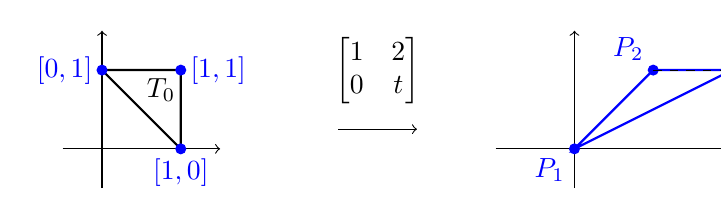
\begin{tikzpicture}[scale=1]

% primo triangolo
% Assi
\draw[->] (-0.5,0) -- (1.5,0);
\draw[->] (0,-0.5) -- (0,1.5);

% Lati
\draw[thick] (0,1) -- (1,1) -- (1,0) -- cycle;

% Punti 
\fill[blue] (0,1) circle (2pt) node[left] {$[0,1]$};
\fill[blue] (1,1) circle (2pt) node[right] {$[1,1]$};
\fill[blue] (1,0) circle (2pt) node[below] {$[1,0]$};

% T0
\node at (0.75,0.75) {$T_0$};

\hspace{1cm}
% matrice
\node at (2.5,1) {$\begin{bmatrix} 1 & 2 \\ 0 & t \end{bmatrix}$};
\hspace{1cm}

% freccia
\draw[->] (1,0.25) -- (2,0.25);

% Assi
\draw[->] (3,0) -- (7.5,0);
\draw[->] (4,-0.5) -- (4,1.5);

% punti 2
\coordinate (P1) at (4,0);
\coordinate (P2) at (5,1);
\coordinate (P3) at (6,1);

% triangolo 2
\draw[thick, blue] (P1) -- (P2) -- (P3) -- cycle;

% Punti
\fill[blue] (P1) circle (2pt) node[below left] {$P_1$};
\fill[blue] (P2) circle (2pt) node[above left] {$P_2$};
\fill[blue] (P3) circle (2pt) node[above right] {$P_3$};

% Linee tratteggiate
\draw[dashed] (P2) -- (6,1);
\draw[dashed] (P3) -- (6,0);

\end{tikzpicture}

\[
A(P_1\Hat{P_2}P_3) = \frac{|t|}{2}, \quad A(T_0) = \frac{1}{2}
\]
\[
\text{det} \left(\begin{bmatrix} 1 & 2 \\ 0 & t \end{bmatrix} \right) = t - 0 = t
\]

\vspace{1cm}
\noindent IDEA: il determinante di una matrice ci indica come cambiano le aree dopo una trasformazione effettuata tramite un prodotto matriciale
\vspace{1cm}

\noindent N.B. Prima di iniziare con il calcolo del determinante è bene osservare la matrice e, se possibile, individuare la scelta di riga/colonna favorevole, cioè quella che minimizza i calcoli da svolgere. \break
Esempio:
\[
    B = \begin{bmatrix}
        9 & 2 & -2 \\
        2 & 2 & 0 \\
        -2 & 0 & 2 \\
    \end{bmatrix}
\]
Sebbene il risultato non dipenda dalla scelta della riga o colonna da fissare, si nota che la scelta di i = 1 ci porta a svolgere più calcoli:
\[ 
    det(B) = b_{11}det(\begin{bmatrix} 2 & 0 \\ 0 & 2 \end{bmatrix}) - b_{12}det(\begin{bmatrix} 2 & 0 \\ -2 & 2 \end{bmatrix}) + b_{13}det(\begin{bmatrix} 2 & 2 \\ -2 & 0 \end{bmatrix}) = 20
\]
Se scegliamo invece i = 2:
\[ 
    det(B) = -b_{21}det(\begin{bmatrix} 2 & -2 \\ 0 & 2 \end{bmatrix}) + b_{22}det(\begin{bmatrix} 9 & -2 \\ -2 & 2 \end{bmatrix}) + b_{23}det(\hat{B_{23}}) = 20
\]
$b_{23} = 0$, dunque non è necessario calcolare $det(\hat{B_{23}})$

\vspace{1cm}
\begin{center}
    Matrici con determinante facile da calcolare
\end{center}
\begin{itemize}
    \item [(i)] se $A \in M_\mathds{K}(n,n)$ ha una riga o colonna composta da soli elementi uguali a 0, allora $det(A) = 0$. \smallbreak
    Infatti, fissando la riga/colonna di soli 0 si ha:
    \[ 
        det(A) = \sum_{i = 1}^{n}(-1)^{i+j}a_{ij}det(\Hat{A}_{ij}) = 0
    \]
    \item [(ii)] se $A \in \mathds{M}_K(n,n)$  ha due righe o due colonne uguali, $det(A) = 0$
\end{itemize}

\newpage

\begin{itemize}
     \item [(iii)] \begin{defn} Una matrice $T \in M_K(n,n)$ si dice \begin{itemize}
        \item [-] \textit{triangolare superiore} se $t_{ij} = 0 \hspace{0.5cm} \forall i < j$
        \item [-] \textit{triangolare inferiore} se $t_{ij} = 0 \hspace{0.5cm} \forall i > j$
     \end{itemize}
     \end{defn}
\end{itemize}

    

\end{document}
